\section{Procedura di codifica con distorsione}
\label{sec:procedure-with-distortion}

Il risultato della Proposizione~\ref{prop:msi-to-wz} ci permette di considerare
il sistema in esame nella situazione in cui la trasmissione di feedforward è
già avvenuta. A seguito del feedforward infatti, sia la BS che lo UT hanno a
disposizione una descrizione del canale di UL quantizzata
\(q(\bm{h}^\mathrm{(U)})\).

A questo punto è possibile sviluppare una procedura di codifica di sorgente per
la trasmissione in feedback, la quale deve consentire alla BS di ricostruire il
canale di DL minimizzando il tasso della trasmissione stessa. Una panoramica di
una possibile procedura è esposta di seguito, corredata da una versione
schematizzata in Figura~\ref{fig:procedure-schema}.

Allo UT, il canale di DL viene anzitutto quantizzato (per la costruzione del
codebook si veda l'Appendice~\ref{app:codebook-design}). In seguito, il
codificatore utilizza un codice di correzione d'errore per codificare
l'informazione sul canale di DL quantizzato. Quindi, un sottoinsieme delle
parole di codice ottenute viene trasmesso alla BS, considerando l'informazione
laterale \(q(\bm{h}^\mathrm{(U)})\) in comune, così da evitare l'invio di
informazioni già note al decodificatore. Alla ricezione, la BS impiega un
decodificatore a decisione morbida (\textit{soft-decision decoder}) per
determinare, con l'aiuto dell'informazione laterale \(\bm{h}^\mathrm{(U)}\), la
stima più probabile del canale di UL \(\hat{\bm{h}}^\mathrm{(D)}\).
\begin{figure}[ht]
    \centering
    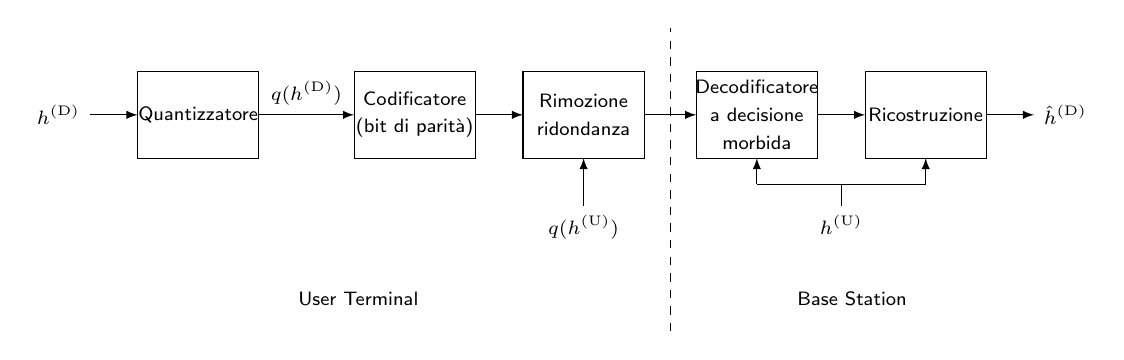
\begin{tikzpicture}[scale=0.55,>=latex]
    \tikzstyle{every node}=[font=\fontsize{6.8}{10}\sffamily]

    % Coding at UT
    \draw[->] (1.1,5) node[left]{\(\bm{h}^\mathrm{(D)}\)} -- (2.2,5);

    \draw (2.2,4) rectangle (5,6)
    node[midway,align=center]{Quantizzatore};

    \draw[->] (5,5) -- (7.2,5)
    node[above,midway]{\(q(\bm{h}^\mathrm{(D)})\)};

    \draw (7.2,4) rectangle (10,6)
    node[midway,align=center]{Codificatore \\ (bit di parità)};

    \draw[->] (10,5) -- (11.1,5);

    \draw (11.1,4) rectangle (13.9,6)
    node[midway,align=center]{Rimozione \\ ridondanza};

    \draw[->] (12.5,2.9) node[below]{\(q(\bm{h}^\mathrm{(U)})\)} -- (12.5,4);

    % Send in Feedback
    \draw[->] (13.9,5) -- (15.1,5);
    \draw[-, dashed] (14.5,0) -- (14.5,7);
    \draw (7.3,0.75) node {User Terminal};
    \draw (18.7,0.75) node {Base Station};

    % Decoding at BS
    \draw (15.1,4) rectangle (17.9,6)
    node[midway,align=center]{Decodificatore \\ a decisione \\ morbida};

    \draw[->] (16.5,3.4) -- (16.5,4);

    \draw[->] (17.9,5) -- (19,5);

    \draw (19,4) rectangle (21.8,6)
    node[midway,align=center]{Ricostruzione};

    \draw[->] (20.4,3.4) -- (20.4,4);

    \draw[-] (16.5,3.4) -- (20.4,3.4);
    \draw[-] (18.45,2.9) node[below]{\(\bm{h}^\mathrm{(U)}\)} -- (18.45,3.4);

    \draw[->] (21.8,5) -- (22.9,5)
    node[right]{\(\hat{\bm{h}}^\mathrm{(D)}\)};
\end{tikzpicture}

    \caption{
        Schema della codifica di sorgente con distorsione per la trasmissione
        del canale di DL in feedback.
    }
    \label{fig:procedure-schema}
\end{figure}
\newline
Il decodificatore a decisione morbida infatti può utilizzare un'informazione a
priori sulla distribuzione delle parole di codice. Questa distribuzione è
ottenuta dalla conoscenza del canale di UL e dalla correlazione di quest'ultimo
con il canale di DL.
